\def\year{2019}\relax
%File: formatting-instruction.tex
\documentclass[letterpaper]{article} % DO NOT CHANGE THIS
\usepackage{aaai19}  % DO NOT CHANGE THIS
\usepackage{times}  % DO NOT CHANGE THIS
\usepackage{helvet} % DO NOT CHANGE THIS
\usepackage{courier}  % DO NOT CHANGE THIS
\usepackage[hyphens]{url}  % DO NOT CHANGE THIS
\usepackage{graphicx} % DO NOT CHANGE THIS
\urlstyle{rm} % DO NOT CHANGE THIS
\def\UrlFont{\rm}  % DO NOT CHANGE THIS
\usepackage{graphicx}  % DO NOT CHANGE THIS
\frenchspacing  % DO NOT CHANGE THIS
\setlength{\pdfpagewidth}{8.5in}  % DO NOT CHANGE THIS
\setlength{\pdfpageheight}{11in}  % DO NOT CHANGE THIS

%PDF Info Is REQUIRED.
% For /Author, add all authors within the parentheses, separated by commas. No accents or commands.
% For /Title, add Title in Mixed Case. No accents or commands. Retain the parentheses.
 \pdfinfo{
/Title (Compiling Cost-Optimal Multi-Agent Pathfinding to ASP)
/Author (Rodrigo N. Gomez, Carlos Hernandez, Jorge A. Baier)
} %Leave this
% /Title ()
% Put your actual complete title (no codes, scripts, shortcuts, or LaTeX commands) within the parentheses in mixed case
% Leave the space between \Title and the beginning parenthesis alone
% /Author ()
% Put your actual complete list of authors (no codes, scripts, shortcuts, or LaTeX commands) within the parentheses in mixed case.
% Each author should be only by a comma. If the name contains accents, remove them. If there are any LaTeX commands,
% remove them.

% DISALLOWED PACKAGES
% \usepackage{authblk} -- This package is specifically forbidden
% \usepackage{balance} -- This package is specifically forbidden
% \usepackage{caption} -- This package is specifically forbidden
% \usepackage{color (if used in text)
% \usepackage{CJK} -- This package is specifically forbidden
% \usepackage{float} -- This package is specifically forbidden
% \usepackage{flushend} -- This package is specifically forbidden
% \usepackage{fontenc} -- This package is specifically forbidden
% \usepackage{fullpage} -- This package is specifically forbidden
% \usepackage{geometry} -- This package is specifically forbidden
% \usepackage{grffile} -- This package is specifically forbidden
% \usepackage{hyperref} -- This package is specifically forbidden
% \usepackage{navigator} -- This package is specifically forbidden
% (or any other package that embeds links such as navigator or hyperref)
% \indentfirst} -- This package is specifically forbidden
% \layout} -- This package is specifically forbidden
% \multicol} -- This package is specifically forbidden
% \nameref} -- This package is specifically forbidden
% \natbib} -- This package is specifically forbidden -- use the following workaround:
% \usepackage{savetrees} -- This package is specifically forbidden
% \usepackage{setspace} -- This package is specifically forbidden
% \usepackage{stfloats} -- This package is specifically forbidden
% \usepackage{tabu} -- This package is specifically forbidden
% \usepackage{titlesec} -- This package is specifically forbidden
% \usepackage{tocbibind} -- This package is specifically forbidden
% \usepackage{ulem} -- This package is specifically forbidden
% \usepackage{wrapfig} -- This package is specifically forbidden
% DISALLOWED COMMANDS
% \nocopyright -- Your paper will not be published if you use this command
% \addtolength -- This command may not be used
% \balance -- This command may not be used
% \baselinestretch -- Your paper will not be published if you use this command
% \clearpage -- No page breaks of any kind may be used for the final version of your paper
% \columnsep -- This command may not be used
% \newpage -- No page breaks of any kind may be used for the final version of your paper
% \pagebreak -- No page breaks of any kind may be used for the final version of your paperr
% \pagestyle -- This command may not be used
% \tiny -- This is not an acceptable font size.
% \vspace{- -- No negative value may be used in proximity of a caption, figure, table, section, subsection, subsubsection, or reference
% \vskip{- -- No negative value may be used to alter spacing above or below a caption, figure, table, section, subsection, subsubsection, or reference

%% Our packages
\usepackage[algoruled,vlined,linesnumbered]{algorithm2e}
\usepackage{amsmath}
\usepackage{amssymb}
\usepackage{latexsym}
\usepackage[usenames,dvipsnames,svgnames,table]{xcolor}
\usepackage{units}
\usepackage{booktabs}

%% Our macros
\newcommand{\jb}[1]{{\small\sf \color{blue} Jorge: #1}}
\newcommand{\ch}[1]{{\small\sf \color{red} Carlos: #1}}
\newcommand{\rg}[1]{{\small\sf \color{orange} Rodrigo: #1}}

\newtheorem{definition}{Definition}
\newtheorem{theorem}{Theorem}
\newtheorem{lemma}{Lemma}
\newtheorem{corollary}{Corollary}

\newcommand{\citea}[1]{\citeauthor{#1}~(\citeyear{#1})}

%%%%%%%%%%%%%%%%%%%%%%%%%%%%%%%%%%%%%%%%%%%%%%%%%%%

%\setcounter{secnumdepth}{2}

% The file aaai19.sty is the style file for AAAI Press
% proceedings, working notes, and technical reports.
%
%\setlength\titlebox{2.5in} % If your paper contains an overfull \vbox too high warning at the beginning of the document, use this
% command to correct it. You may not alter the value below 2.5 in
\title{Compiling Cost-Optimal Multi-Agent Pathfinding to ASP}
%Your title must be in mixed case, not sentence case.
% That means all verbs (including short verbs like be, is, using,and go),
% nouns, adverbs, adjectives should be capitalized, including both words in hyphenated terms, while
% articles, conjunctions, and prepositions are lower case unless they
% directly follow a colon or long dash
\author{Rodrigo N.\ G\'omez,\textsuperscript{\rm 1}  Carlos Hern\'andez,\textsuperscript{\rm 2}  Jorge A.\ Baier\textsuperscript{\rm 1,3} \\
\textsuperscript{\rm 1} Departamento de Ciencia de la Computaci\'on, Pontificia Universidad Cat\'olica de Chile, Santiago, Chile \\
\textsuperscript{\rm 2} Departamento de Ciencias de la Ingenier\'ia, Universidad Andr\'es Bello, Santiago, Chile\\
\textsuperscript{\rm 3} Instituto Milenio Fundamentos de los Datos, Chile}
%\author{Written by AAAI Press Staff\textsuperscript{\rm 1}\thanks{Primarily Mike Hamilton of the Live Oak Press, LLC, with help from the AAAI Publications Committee}\\ \Large \textbf{AAAI Style Contributions by
%Pater Patel Schneider,} \\ \Large \textbf{Sunil Issar, J. Scott Penberthy, George Ferguson, Hans Guesgen}\\ % All authors must be in the same font size and format. Use \Large and \textbf to achieve this result when breaking a line
%\textsuperscript{\rm 1}Association for the Advancement of Artificial Intelligence\\ %If you have multiple authors and multiple affiliations
% use superscripts in text and roman font to identify them. For example, Sunil Issar,\textsuperscript{\rm 2} J. Scott Penberthy\textsuperscript{\rm 3} George Ferguson,\textsuperscript{\rm 4} Hans Guesgen\textsuperscript{\rm 5}. Note that the comma should be placed BEFORE the superscript for optimum readability
%2275 East Bayshore Road, Suite 160\\
%Palo Alto, California 94303\\
%publications19@aaai.org % email address must be in roman text type, not monospace or sans serif
%}


\newcommand{\Up}{\ensuremath{\mathit{up}}}
\newcommand{\Down}{\ensuremath{\mathit{down}}}
\newcommand{\Left}{\ensuremath{\mathit{left}}}
\newcommand{\Right}{\ensuremath{\mathit{right}}}
\newcommand{\Wait}{\ensuremath{\mathit{wait}}}



 \begin{document}

\maketitle

%\begin{abstract}
%Multi-Agent Pathfinding (MAPF) over grids is the problem of finding n non-conflicting paths that lead n agents from a given initial cell to a given goal cell. Cost-optimal MAPF in addition minimizes the total number of actions performed by each agent before stopping at the goal. Being a combinatorial problem in nature, a number of compilations from MAPF to Answer Set Programming (ASP) exist. In this paper we propose a new one, which unlike existing ASP approaches (1) produces cost-optimal solutions, and (2) exploits heuristics that can be pre-computed quickly using Dijkstra's algorithm. Like makespan-optimal approaches, our algorithm searches for solutions with increasing makespan. When a solution is found, rather than returning it, it computes a (provably correct) upper bound on the maximum makespan at which a true cost-optimal solution exists, and reruns the solver in search for such a solution. In our empirical evaluation, in which we use the clasp solver, we show that by exploiting parallelism our approach is competitive with search-based state-of-the-art algorithms on small grids.
%\end{abstract}

\section{Introduction}
Multi-Agent Pathfinding (MAPF) over grids is the problem of finding $n$ non-conflicting paths that lead $n$ agents from a given initial cell to a given goal cell. Sum-of-costs-optimal MAPF, or simply cost-optimal MAPF, in addition, minimizes the total number of actions performed by each agent before stopping at the goal. Being a combinatorial problem in nature, a number of compilations from MAPF to Satisfiability (SAT) \cite{SurynekFSB16} and Answer Set Programming (ASP) exist \cite{ErdemKOS13,GebserOOS18}. Here we propose and evaluate a new compilation of MAPF over grids to ASP. Unlike existing compilations we are aware of, both to SAT and to ASP, our encoding is the first that produces a number of clauses that is \emph{linear} on the number of agents. In addition, the clauses that allow representing the optimization objective are also efficiently written, and do not depend on the size of the grid. Like makespan-optimal approaches, our algorithm searches for cost-optimal solutions with increasing makespan. When a solution is found a provably correct upper bound on the maximum makespan at which a true cost-optimal solution exists is computed, and the solver is rerun once more.


\section{Answer-Set Programming}
Answer-set programming (ASP) \cite{Lifschitz08} is a logic-based framework for knowledge reasoning and constraint optimization. Optimization problems are modeled with an ASP \emph{program} over a set of \emph{atoms} $\mathcal{P}$, such that a \emph{model} of the program, which is a subset of $\mathcal{P}$, encodes an optimal solution. An ASP program can be viewed as composed by a set of rules \emph{rules}, a set of \emph{constraints}, and \emph{optimization statements}.  Each rule specifies under which conditions certain atoms should become part of the model. In our compilation, we use two types of rules. The first type are \emph{basic rules}, that have the form $p\leftarrow B$, where $p\in \mathcal{P}$ and $B\subseteq \mathcal{P}$, which intuitively specify that when all atoms in $B$ are part of a model, so is $p$. The second type, henceforth referred to as \emph{singleton rules}, have the form $1=|A|\leftarrow B$, where $A,B\subseteq \mathcal{P}$, and specify that whenever $B$ is contained in the model, only one element of $A$ should be.
Constraints of the form $\leftarrow C$, where $C\subseteq \mathcal{P}$, express $C$ cannot be contained in a model. Finally an optimization statement, of the form $min A$ (resp. $max A$) instructs the solver to minimize (resp. maximize) the number of atoms in $A$ that appear in the model.

\begin{figure*}
    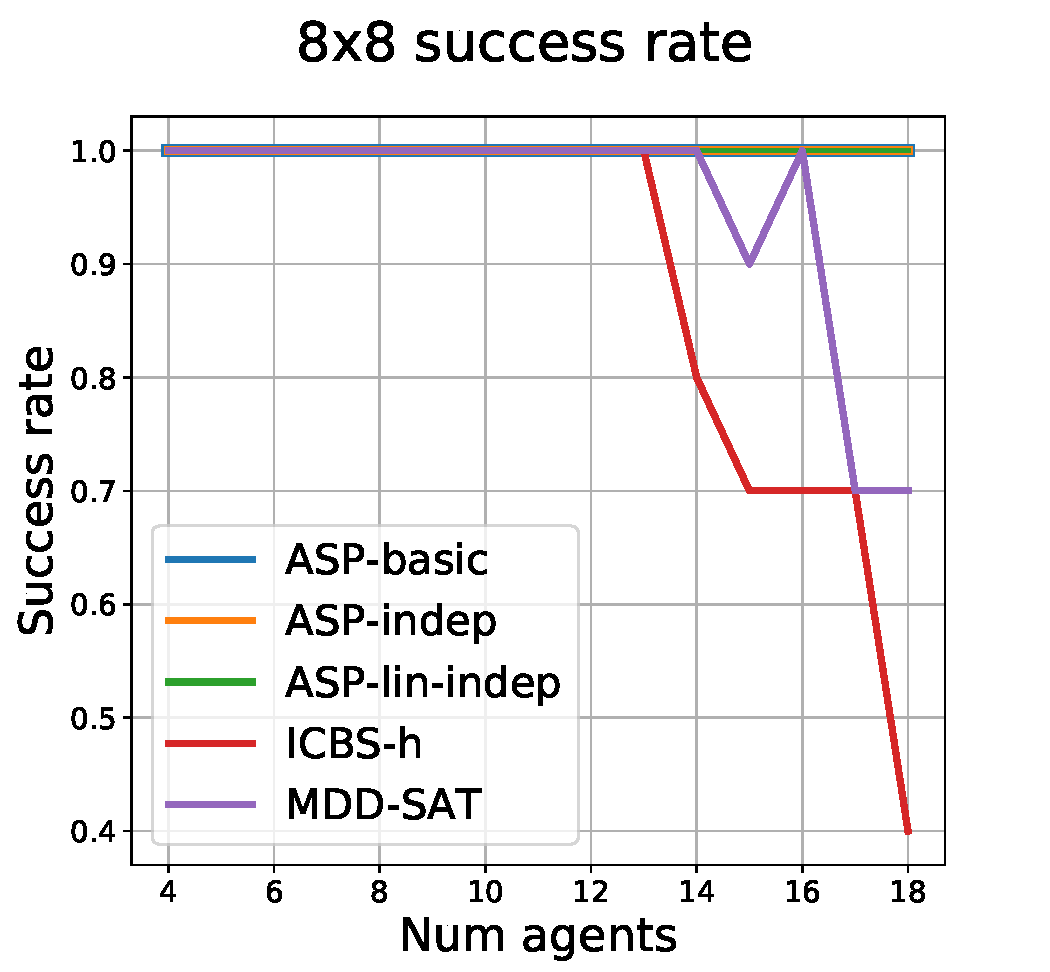
\includegraphics[width=0.24\textwidth]{graphs/8x8succ.pdf}
    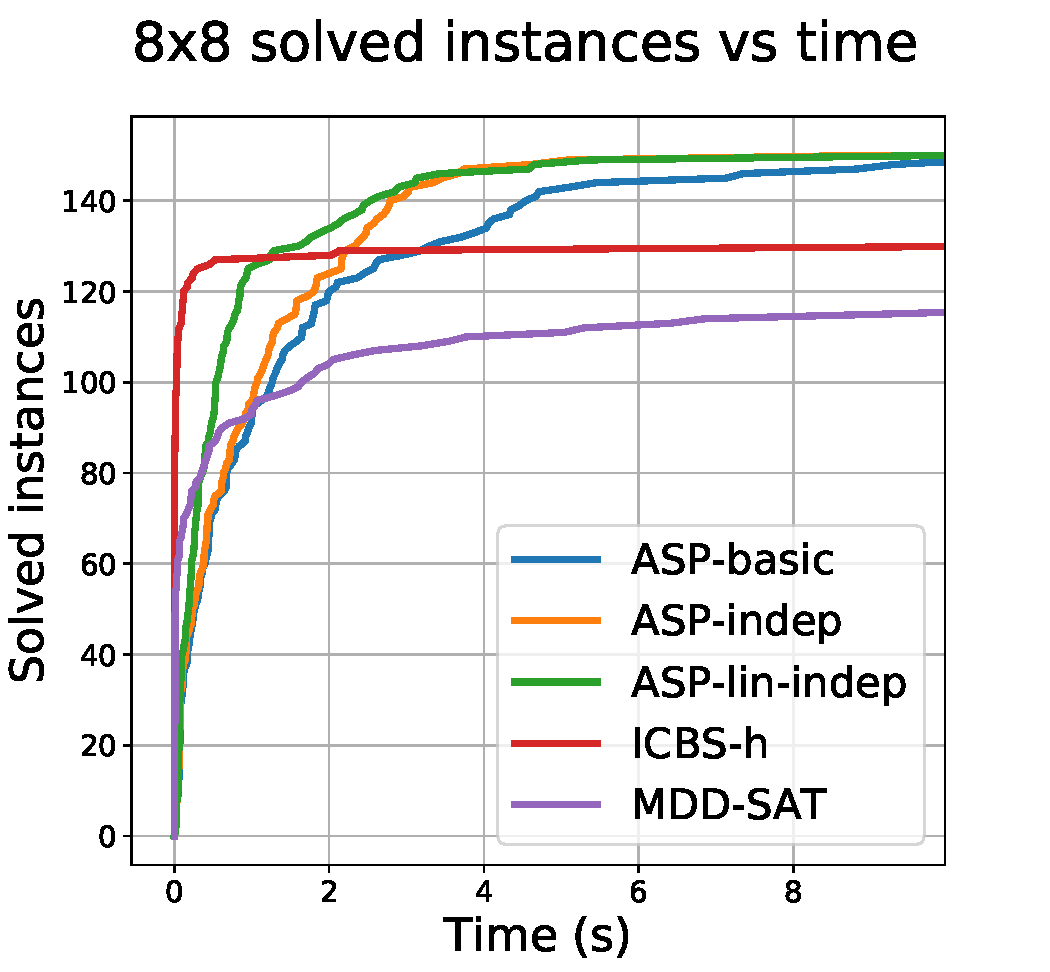
\includegraphics[width=0.24\textwidth]{graphs/8x8runtime.pdf}
    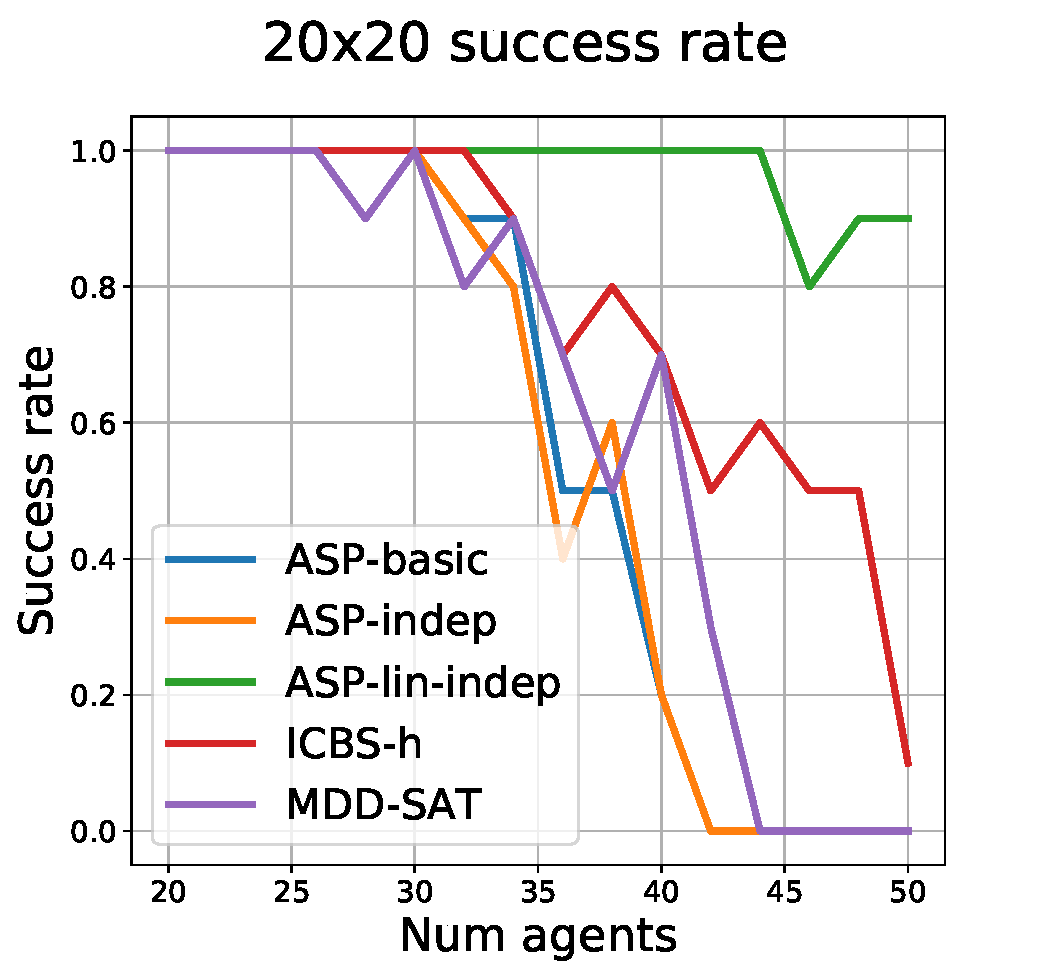
\includegraphics[width=0.24\textwidth]{graphs/20x20succ.pdf}
    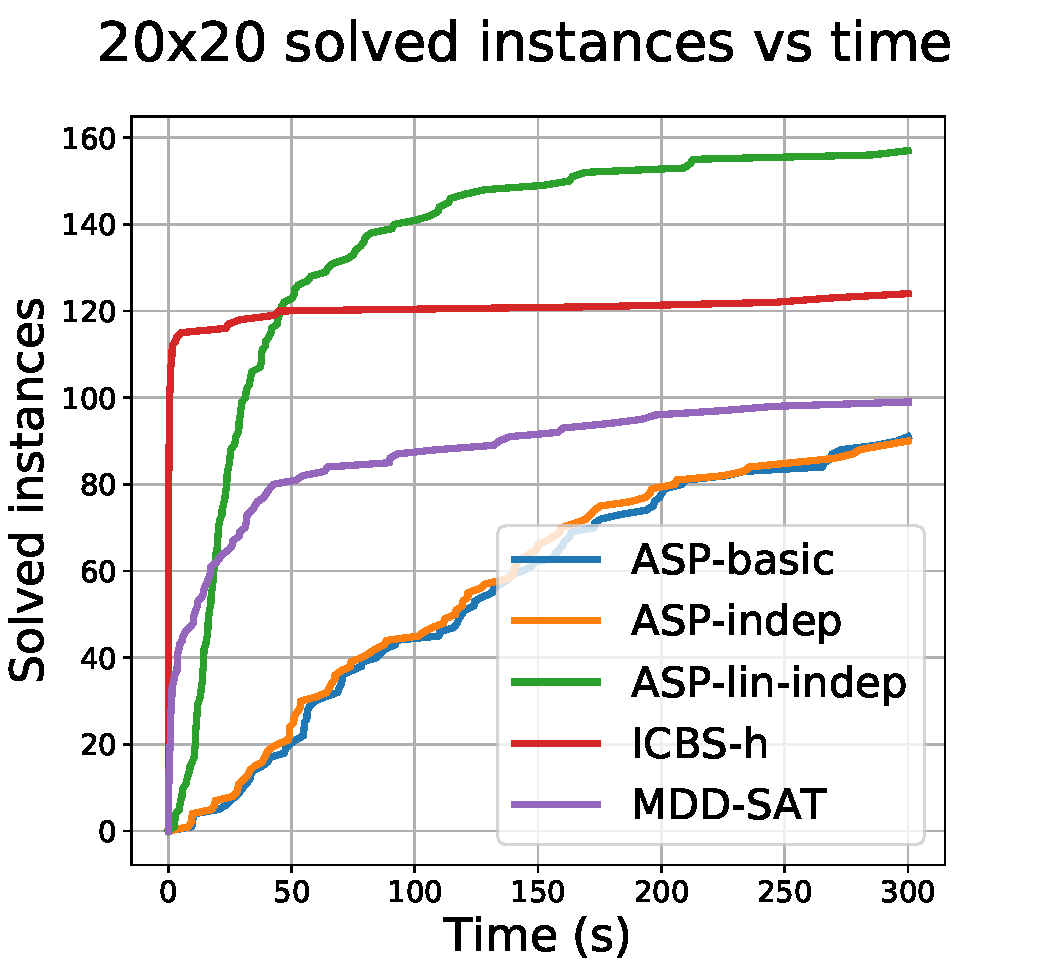
\includegraphics[width=0.24\textwidth]{graphs/20x20runtime.pdf}
    \caption{Success rate and number of instances solved versus time on $8\times 8$ and $20\times 20$ grids.}
    \label{figure}
\end{figure*}


\section{From MAPF to ASP}
Like compilations of planning to satisfiability, we use atoms of the form $at(a,x,y,t)$ to specify that an agent $a$ is at cell $(x,y)$ at \emph{time instant} $t$, and our encoding considers instances of these atoms for $t$ between $0$ and $T$, where $T$ is the makespan of the solution sought. Atoms of the form $exec(a,m,t)$ specify that agent $a$ executes $m$ at time $t$.

\noindent\textbf{Effects of moves} To encode the effect of agent $a$ performing move $m$ we use a basic rules of the form $at(a,x,y,t+1)\leftarrow at(a,x',y',t),exec(a,m,t)\cup B$, where $B$ specifies the way $(x,y)$ and $(x',y')$ are related depending on $m$.

\noindent\textbf{Parallel move execution} To encode that each agent performs exactly one move at each time instant, we use singleton rules, expressing that set $\{exec(a,m,t):m\in Moves\}$ has cardinality 1 for each agent $a$ and each time instant $t$.

\noindent\textbf{Conflict avoidance} Here we want to express that the paths do not have conflicts. We need to express that (1) no pair of different agents are ever at the same cell and (2) there is no pair of adjacent agents that \emph{swap} cells after performing a single (parallel) move. We do this by adding constraints to the program. We experimented with two approaches.

\noindent \emph{Quadratic conflict encoding}. The first approach is similar to what is done in MDD-SAT \cite{SurynekFSB16} and ASPRILO \cite{GebserOOS18}.  We write the constraints $\leftarrow {on(a,x,y,t),on(a',x,y,t)}$, for every pair of different agents $(a,a')$, every time instant $t$, and every grid cell $(x,y)$. Similarly, we write constraints for disallowing swaps; these are omitted for space, but we need one for each pair of different agents. This yields a representation that is quadratic on the number of agents, and linear on the size of the map.

\noindent \emph{Linear conflict encoding}. Here we introduce atoms of the form $rt(x,y,t)$ to specify that the edge between $(x,y)$ and $(x+1,y)$ is traversed by \emph{some} agent at time $t$. $lt(x+1,y,t)$, on the other hand, represents that an agent moved from  $(x+1,y)$ to $(x,y)$ a time $t$. In addition, atom $st(x,y,t)$ represents some agent at $(x,y)$ at time $t$ performed a wait action at $t$. The dynamics of these predicates are defined using basic rules like $lt(x,y,t)\leftarrow exec(a,\mathrm{right},t),on(a,x,y,t)$ for every agent $a$, cell $(x,y)$, and time instant $t$. Their definition is thus linear in the number of agents and the size of the grid. Finally, for swaps, we express constraints like $\leftarrow rt(x,y,t),lr(x+1,y,t)$ for every $(x,y)$ in the grid, and time instant $t$. The resulting number of constraints and rules is linear in the size of the map.


\noindent \textbf{Optimization} To find a cost-optimal solution, we need to encode the minimization of the number of actions executed by the agents. We tried with two different encodings.

\noindent \emph{Grid-dependent penalty}. This encoding is similar to the approach used in MDD-SAT: the idea to minimize the actions performed by the agent at each cell. Specifically there is an atom $cost(a,t,1)$ which specifies that agent $a$ has performed an action at time $t$. To define this atom, we need to specify three rule schemas. One of them is $cost(a,t,1) \leftarrow on(a,x,y,t), notgoal(a,x,y)$, which establishes that moving the agent from a cell that is not the goal is penalized by one unit. There are three more rule types that we omit for space. The resulting number of rules and constraints grows linearly with the size of the grid and the number of agents. Finally, via an optimization statement, we minimize the number of atoms of the form $cost(a,t,1)$ in the model.

\noindent \emph{Grid-independent encoding}. Here we maximize the slack between the makespan $T$ and the time instant at which an agent has stopped at the goal. We define atoms of the form $at\_goal\_back(a,t)$ which specify that between time instants $t$ and $T$ agent $a$ is at the goal. The rule defining these atoms ensures that no action other than wait has been performed between $t$ and $T$, without making reference to the cells int the grid, resulting in an encoding that does not depend on the grid, and thus is linear in the number of agents.

\noindent \textbf{Achieving the goal} Via a constraint, we specify that no agent is away from its goal at time $T$.

\noindent \textbf{Obtaining an optimal solution} Let $T_0$ and $C_0$ be, respectively, the makespan and cost of the solution that is obtained by solving the problem independently for each agent, ignoring all others. To obtain an optimal solution we iterate from $T=T_0$ incrementing $T$ by one until a solution is found. Now let $T_0$ and $C_0$ be, respectively, the makespan and cost of the first solution found. Then we run the solver for one last time with makespan $T_1+C_1-1-C_0$, which we can prove will return an optimal solution.

%\section{Cost-Optimal MAPF to ASP Given a Makespan}
In this section we describe two cost-optimal encodings for MAPF to ASP for a given makespan $m$. As such, when given to an ASP solver, they will generate a cost-optimal solution which does not exceed makespan $m$. In the next section, we show that these solutions are not necessarily truly cost-optimal. For now however, we focus on this simpler case to ease our presentation.

The first is a straightforward encoding that states that each time the agent performs an action away from the goal state, then $penalty(R,t,1)$ holds true.

\begin{align*}
penalty(R,t,1) \leftarrow &at(R,X,Y,t), not\: goal(R,X,Y). \\
penalty(R,t,1) \leftarrow &at(R,X,Y,t), goal(R,X,Y), exec(R,A,t),A!=wait. \\
penalty(R,t,1) \leftarrow &goal(R,X,Y), at(R,X,Y,t), exec(R,wait,t), not\: at\_goal\_back(R,t). \\
at\_goal\_back(R,m) \leftarrow &robot(R). \\
at\_goal\_back(R,T-1) \leftarrow &tiempo(t),at\_goal\_back(R,t),exec(R,wait,t-1). 
\end{align*}

%%\section{Makespan as a Bound}
% To guarantee that our model will yield a solution that is \emph{sum-of-costs} optimal we need to provide a maximum $makespan$ $T$ big enough.

% In figure , we show an example where the increase of the \emph{makespan} returns better \emph{sum-of-costs} solutions. The problem has 3 agents:  $a_1$ needs to go from $(0,1)$ to $(3,1)$. The agents $a_2$ and $a_3$ are already at the goal on the positions $(1,1)$ and $(2,1)$ respectively. We compare the minimum \emph{sum-of-costs} solution with two different \emph{makespans}:

% \begin{itemize}
%     \item $\mu=3$. The optimal \emph{sum-of-costs} solution involves moving $a_2$ and $a_3$ out of their goal. The costs for each agent are: $cost(a_1) = 3$, $cost(a_2) = 2$ and $cost(a_3) = 3$, which gives us \emph{sum-of-costs} $=8$.
%     \item $\mu=5$. The optimal \emph{sum-of-costs} solution only needs to move $a_1$, dodging the locations occupied by the other agents: \emph{sum-of-costs} $=cost(a_1) = 5$
% \end{itemize}



% \emph{makespan} $m_{opt}$ that guarantees a cost-optimal solution given an initial solution.

% \begin{lemma}
% Given an initial solution with cost $\sigma$. We can bound $m_{opt}$ as:
% \[
%     m_{opt} \leq  \sigma - \min\limits_{i=\{1..k\} }{\sum_{\substack{j=1 \\ j \neq i}}^{k} c^*(a_j)}
% \]
% Where $c^*(a_j)$ is the optimal cost of the path $a_j$ ignoring the conflicts with other agents.
% \end{lemma}

\subsection{Finding Cost-Optimal Solutions}
The encoding proposed so far can find the minimum sum-of-cost solution for a given makespan. We still need to define how to find a true cost-optimal solution.

Following the approach used for SAT encodings for planning \cite{KautzS92}, in our approach we attempt to solve instances for increasing makespan $\mathtt{T}$, until a solution, say $sol_{min}$, is found. Two observations with this process are important. First, we do not need to start increasing $\mathtt{T}$ from 1. As mentioned above, at preprocessing time, for each agent we compute cost the cost $c^*_a$ which ignores other agents. The makespan of any solution must be at least $\max_{a\in\mathcal{A}} c^*_a$ so this can be the inferior limit of our iteration.

Second, let $sol_{min}$ be the solution that is found first. Unfortunately, $sol_{min}$ is a makespan-optimal solution but not necessarily a cost-optimal solution. Now we can compute a bound for the largest makespan $\mathtt{T}_{max}$ at which the cost-optimal solution is found, using the following theoretical result first proposed by \acite{SurynekFSB16}:
\begin{theorem}[\nbcite{SurynekFSB16}]\label{thm:optimal}
Let $sol_{min}$ be the makespan-optimal solution for MAPF problem $P$, let $sol^-$ denote a solution to $P$ that ignores all conflicts, and let $\mathtt{T}^-$ denote its makespan. Then the makespan of the cost-optimal solution is at most at $\mathtt{T}_{max}=\mathtt{T}^- + c(sol_{min})-c(sol^-)-1$.
\end{theorem}
Thus after we find the first solution $sol_{min}$, we run the solver again for makespan $\mathtt{T}_{max}$ given by Theorem~\ref{thm:optimal}. The approach described in this section was recently evaluated by \acite{BartakS19} for their Picat-based MAPF solver.


%First we calculate the shortest path for each agent ignoring the conflicts with other agents. The maximum cost and sum of costs of these paths provide a lower bound for the makespan $\mathtt{T}_{min}$ and \emph{sum-of-costs} respectively. Then we define and start solving an ASP program with one of the encodings defined before using $\mathtt{T}=\mathtt{T}_{min}$ as the makespan. If there's no solution we increase $\mathtt{T}$ by 1 and repeat the process.

%If the program returns a valid solution then as it was shown in Figure ~\ref{fig:makespancost} it's not guaranteed that is \emph{sum-of-cost} optimal.

%The using (bartak)

%So we run the program one last time using $\mathtt{T}=C(M) - 1 - C^-$ and return that solution.


% \begin{algorithm}
% \DontPrintSemicolon
% \KwIn{A MAPF problem}
% $\mathtt{T} \gets \max\limits_{i=\{1..K\} }{c^*(a_i)}$\;
% $C^- \gets \sum_{\substack{i=1}}^{k} c^*(a_i)$\;
% $P(\mathtt{T}) \gets$ Create an ASP program from input problem with makespan T\;% $M \gets \{\}$\;
%  \While{$M$ is empty}{%
%   $M \gets$ Solve $P(T)$\;
%   \If{$M$ is not empty}{
%     $C(M) \gets$ cost of the solution of model $M$\;
%     $\Delta \gets C(M) - 1 - C^-$\;
%     $M^* \gets$ Solve $P(\mathtt{T}+\Delta)$\;
%     \Return{M}\;
%   }
%   $\mathtt{T} \gets \mathtt{T}+1$\;
 %}

%\end{algorithm}



\section{Empirical Evaluation}
The objective of our preliminary evaluation was to evaluate combinations of our encodings and compare them to publicly available search-based solvers as well as MDD-SAT \cite{Surynek14} (enc=mdd), on congested grids. We ran two state-of-the-art search algorithms:  EPEA* \cite{Goldenberg14}, and ICBS-h \cite{FelnerLB00KK18}, but decided just to report on the latter, since it was the best performing.

We used Clingo 5.3 as the underlying ASP solver. Clingo was run with 4 threads in \textit{parallel-mode}, and using \textit{usc} as the optimization strategy. 
%We used the implementations by their authors: C++ for MDD-SAT and C\# for ICBS-h. 
Experiments were run on a 3.40GHz Intel Core i5-3570K computer with 8GB of memory. We set a runtime limit of 5 minutes for all the problems.

We experimented on $8\times 8$ and $20\times 20$ randomly generated problems with 10\% obstacles. For $8\times8$ (resp.~$20\times 20$) we generate 150 (resp.~160) problems with the number of agents in $\{4,\dots,18\}$ (resp.~$\{20,22,\ldots,50\}$). Success rates, and number of problems solved versus time are shown in Figure~\ref{figure}, where ASP-basic is a basic encoding that uses quadratic conflict resolution and grid dependent penalties. ASP-indep uses quadratic conflict resolution and grid independent penalties. Finally, ASP-lin-indep uses linear conflict resolution and grid independent penalties. We conclude that in congested grids, ASP-lin-indep is superior to both search-based the other compilation-based approaches. 
%\section{Empirical Evaluation}

%\section{Conclusions and Future Work}
We proposed a compilation to ASP that produces cost-optimal solutions, which is competitive with other state of the art algorithms on congested grids.

Future research will be focused on different aspects:
\begin{itemize}
    \item Because the grounding process takes a lot of time in the algorithm, we will research alternatives to execute the \emph{grounding}. This can mean doing this process manually.
        
    \item Research the possibility on making a sub optimal solver based on our encodings. Debido a los alentadores resultados mostrados en grillas pequeñas es que podríamos integrar nuestro solver a otros algoritmos como Windowed Hierarchical Cooperative A*. De esta manera podemos aprovechar los beneficios de los algoritmos basados en busqueda en grillas de gran tamaño  y los beneficios de nuestra codificación en problemas compactos.

\end{itemize}

\footnotesize
\bibliographystyle{aaai}
\bibliography{ref}

\end{document}
